\chapter{Benutzeroberfläche}

Grundlegend ist die Benutzeroberfläche in drei Web-Seiten unterteilt:
Zunächst die Anfangsseite, von der alle anderen Aktionen gestartet werden können.
Das Seitenlayout ist wie folgend geplant:


\section{/B10/ Seitenlayout}

 \begin{itemize}
   \item Bibliothek
   \begin{itemize}
    \item Suche
      \begin{description}
       \item[Einfache Suche] Die einfache Suche soll intuitiv funktionieren, sie besteht lediglich aus einer Eingabefläche, worin der Benutzer
       Dokumenttitel, Autoren oder Sonstiges eingeben kann. 
       \item[Erweiterte Suche] Die erweiterte Suche stellt dem anspruchsvolleren Anwender mehrere Eingabeflächen zur Verfügung, um gezielter suchen zu können 
       \end{description}
      \item Rückgabe
      \item (Eintragen)(nur vorhanden, falls als Bibliothekar eingeloggt; für weitere Informationen s. Nutzergruppen)
      \item Einloggen
    \end{itemize}
    \item Literaturverzeichnis
    \item Administration
 \end{itemize}
 
\begin{figure}
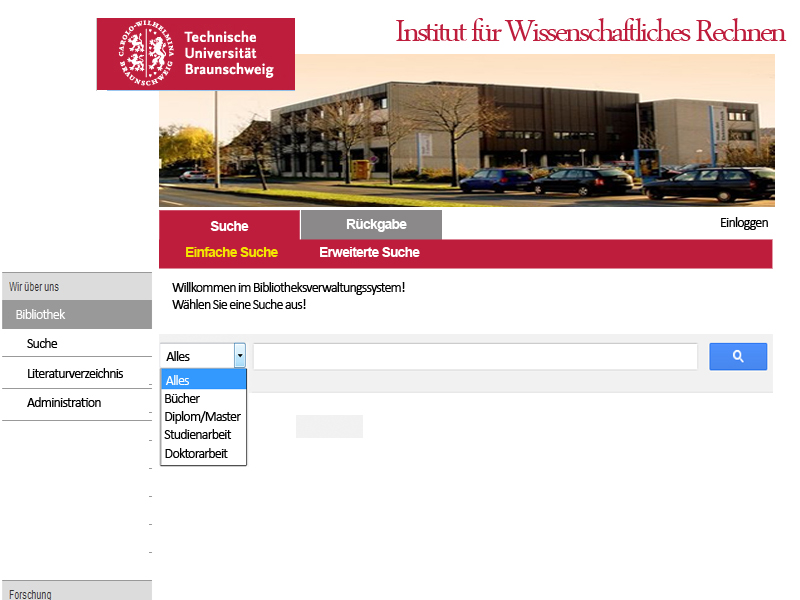
\includegraphics[width=0.8\linewidth]{bilder/layout2.jpg}
\caption{Beispiel für ein Seitenlayout}
\end{figure}

Suchergebnisse werden in einem großen Bereich rechts bzw. unter der Navigation angezeigt. Die Dokumente werden übersichtlich in tabellenartiger Form bereitgestellt. Bei einem Klick auf ein Dokument des Suchergebnisses erscheinen genauere Informationen über das Dokument (Titel,Autor,Jahr etc.), sowie
seinen Status (ausgeliehen, vorhanden, verloren).
Oben rechts wird zudem der eingeloggte User angezeigt.
Bei einem Klick auf den eingeloggten User ist eine Account-Verwaltungsseite geplant.



\section{/B20/ Account-Verwaltungsseite}
  	 	
Hier kann der Benutzer seinen Account verwalten, d.h. er/sie kann die persönlichen Daten und die E-Mail Adresse ändern.
Zusätzlich gibt es hier eine Liste alle Dokumente, welche der eingeloggte User zu eben diesem Zeitpunkt ausgeliehen hat.



\section{/B30/ Administration}

Nur der Administrator hat auf diese Schaltfläche Zugriff, bei allen anderen Nutzern mit weniger Rechten wird eine Fehlermeldung ausgegeben.
Hier kann der Administrator grundlegende Systemeinstellungen ändern und Benutzern Rechte zuweisen.



\section{/B40/ Nutzergruppen}

Darüber hinaus sind mehrere Nutzergruppen geplant(falls nicht anders angegeben, sind die Rechte vom Gast bis zum Administrator aufsteigend additiv zunehmend, d.h. ein Bibliothekar kann neue Dokumente einpflegen, ein Administrator kann dieses auch, aber hat zudem die Möglichkeit Rechte zuzuweisen etc.) 

\begin{description}
\item[Besucher] Wenn ein Nutzer unangemeldet die Seite betritt bzw. auf der Seite ist, gilt er als Besucher(Siehe Abbildung).
\item [\Gls{glos:ext}] Ein Externer ist ein Benutzer, welcher sich nicht anmelden kann. Er wird nur intern verwaltet und hat deswegen die gleiche Sicht
auf das Webinterface wie ein Besucher.
\item [Normaler Benutzer] Als normaler Benutzer gilt ein angemeldeter Benutzer ohne besondere Rechte. Er hat die Möglichkeit, sich Dokumente auszuleihen, und hat Zugriff auf seine eigene Account-Verwaltungsseite.
\item [Bibliothekar] Ein Bibliothekar hat erste Verwaltungsrechte. Ist ein Benutzer als Bibliothekar angemeldet, verändert sich die Navigation des Webinterfaces. Es erscheint zusätzlich eine Schaltfläche „Eintragen“, womit er/sie neue Dokumente in die Bibliothek einpflegen kann.
\item [Verwaltung] Ein Benutzer mit Verwaltungsrechten kann neue Benutzer anlegen und sie bearbeiten.
\item [Administrator] Der Administrator schließlich hat die Möglichkeit, über eine geplante erscheinende Schaltfläche „Administration“, Rechte zu verteilen, d.h. er kann zum Beispiel normalen Benutzern Verwaltungsrechte zuteilen oder entziehen. 
\end{description}











 
